\iffalse
\chapter{2022}
\author{EE24BTECH11037}
\section{me}
\fi


%\begin{enumerate}
    \item After playing \underline{\hspace{1.5cm}} hours of tennis, I am feeling \underline{\hspace{1.5cm}} tired to walk back.
    \begin{enumerate}
        \item too / too
        \item too / two
        \item two / two
        \item two / too
    \end{enumerate}
    \item The average of monthly salaries of $M$, $N$ and $S$ is $Rs.4000$. The average of the monthly salaries of $N,S$ and $P$ is $Rs.5000$. The monthly salary of $P$ is $Rs.6000$. What is the monthly salary of $M$ as a percentage of the monthly salary of $P$?
    \begin{enumerate}
        \item $50\%$
        \item $75\%$
        \item $100\%$
        \item $125\%$
    \end{enumerate}
    \item A person travelled $80km$ in $6$ hours. If the person travelled the first part with a uniform speed of $10kmph$ and the remaining part with a uniform speed of $18 kmph$.\\What percentage of the total distance is travelled at a uniform speed of $10kmph$?
    \begin{enumerate}
        \item $28.25$
        \item $37.25$
        \item $43.75$
        \item $50.00$
    \end{enumerate}
    \item Four girls $P,Q,R$ and $S$ are studying languages in a University. $P$ is learning french and Dutch. $Q$ is learning Chinese and Japanese. $R$ is learning Spanish and French. $S$ is learning Dutch and Japanese.\\Given that: French is easier than Dutch; Chinese is harder than Japanese; Dutch is easier than Japanese, and Spanish is easier than French.\\Based on the above information, which girl is learning the most difficult pair of languages?
    \begin{enumerate}
        \item $P$
        \item $Q$
        \item $R$
        \item $S$
    \end{enumerate}
    \item 
    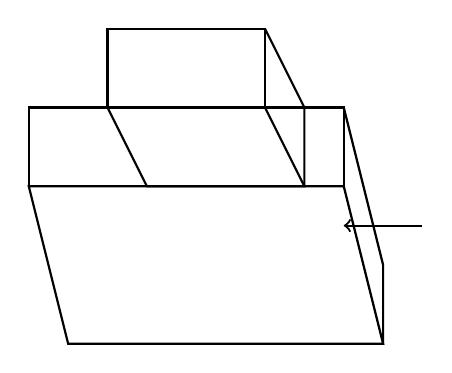
\begin{tikzpicture}
    % Draw the bottom rectangular prism
    \draw[thick] (0, 0) -- (4, 0) -- (3.5, 2) -- (-0.5, 2) -- cycle;
    \draw[thick] (-0.5, 2) -- (-0.5, 3) -- (3.5, 3) -- (3.5, 2);
    \draw[thick] (4, 0) -- (4, 1) -- (3.5, 3);
    \draw[thick] (3.5, 2) -- (3.5, 3);
    
    % Draw the top rectangular prism
    \draw[thick] (1, 2) -- (3, 2) -- (2.5, 3) -- (0.5, 3) -- cycle;
    \draw[thick] (0.5, 3) -- (0.5, 4) -- (2.5, 4) -- (2.5, 3);
    \draw[thick] (3, 2) -- (3, 3) -- (2.5, 4);

    % Draw the arrow
    \draw[->, thick] (4.5, 1.5) -- (3.5, 1.5);

\end{tikzpicture}A block with a trapezoidal cross-section is placed over a block with rectangular cross section as shown in figure.\\Which of the following is the correct drawing of the view of the $3D$ object as viewed in the direction indicated by an arrow in the figure?\\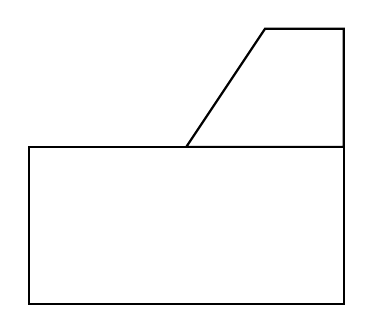
\begin{tikzpicture}
   
    % Draw the bottom rectangle
    \draw[thick] (0, 0) -- (4, 0) -- (4, 2) -- (0, 2) -- cycle;
    
    % Draw the top trapezoid on the right end of the rectangle
    \draw[thick] (2.5, 2) -- (4, 2) -- (4, 3.5) -- (3, 3.5) -- (2, 2) -- cycle;
\end{tikzpicture}
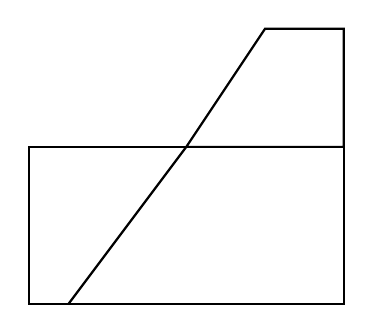
\begin{tikzpicture}
    b)
    % Draw the bottom rectangle
    \draw[thick] (0, 0) -- (4, 0) -- (4, 2) -- (0, 2) -- cycle;
    
    % Draw the top trapezoid on the right end of the rectangle
    \draw[thick] (2.5, 2) -- (4, 2) -- (4, 3.5) -- (3, 3.5) -- (2, 2) -- cycle;

    \draw[thick] (2,2) -- (0.5,0) -- cycle;

\end{tikzpicture}
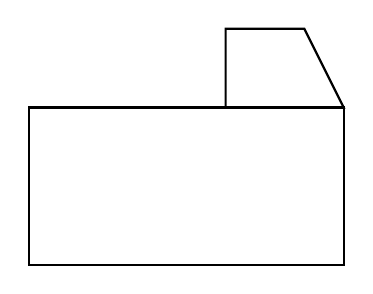
\begin{tikzpicture}

    % Draw the bottom rectangle
    \draw[thick] (0, 0) -- (4, 0) -- (4, 2) -- (0, 2) -- cycle;
    
    % Draw the top trapezoid on the right end of the rectangle
    \draw[thick] (2.5, 2) -- (4, 2) -- (3.5, 3) -- (2.5, 3) -- cycle;

\end{tikzpicture}
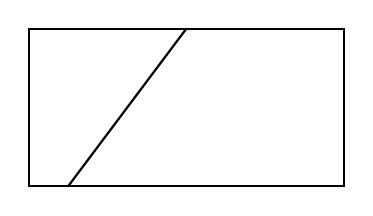
\begin{tikzpicture}
    
    % Draw the bottom rectangle
    \draw[thick] (0, 0) -- (4, 0) -- (4, 2) -- (0, 2) -- cycle;

    \draw[thick] (2,2) -- (0.5,0) -- cycle;

\end{tikzpicture}

     $\brak{1}$ \hspace{1cm} $\brak{2}$ \hspace{1cm} $\brak{3}$ \hspace{1cm} $\brak{4}$

    \item Humans are naturally compassionate and honest. In a study using strategically placed wallets that appear "lost", it was found that wallets with money are more likely to be returned than wallets without money. Similarly, wallets that had a key and money are more likely to be returned than wallets with the same amount of money alone. This suggests that the primary reason for this behavior is compassion and empathy.\\Which one of the following is the CORRECT logical inference based on the information in the above passage?
    \begin{enumerate}
        \item Wallets with a key are more likely to be returned because people do not care about money
        \item Wallets with a key are more likely to be returned because people relate to the suffering of others
        \item Wallets used in experiments are more likely to be returned than wallets that are really lost 
        \item Money is always more important than keys
    \end{enumerate}

    \item A rhombus is formed by joining the midpoints of the sides of a unit square. What is the diameter of the largest circle that can be inscribed within the rhombus?
    \begin{enumerate}
        \item $\frac{1}{\sqrt{2}}$
        \item $\frac{1}{2\sqrt{2}}$
        \item $\sqrt{2}$
        \item $2\sqrt{2}$
    \end{enumerate}
    \item An equilateral triangle, a square and a circle have equal areas.\\What is the ratio of parameters of the equilateral triangle to square to circle?
    \begin{enumerate}
        \item $3\sqrt{3} : 2 : \sqrt{\pi}$
        \item $\sqrt{(3\sqrt{3})} : 2 : \sqrt{\pi}$
        \item $\sqrt{(3\sqrt{3})} : 4 : 2\sqrt{\pi}$
        \item $\sqrt{(3\sqrt{3})} : 2 : 2\sqrt{\pi}$
    \end{enumerate}
    \item Given below are three conclusions drawn based on the following three statements.\\
Statement 1: All teachers are professors.\\
Statement 2: No professor is a male.\\
Statement 3: Some males are engineers.\\

Conclusion I: No engineer is a professor.\\
Conclusion II: Some engineers are professors.\\
Conclusion III: No male is a teacher.\\

Which one of the following options can be logically inferred? 
    \begin{enumerate}
        \item Only conclusion III is correct
        \item Only conclusion I and conclusion II are correct
        \item Only conclusion II and conclusion III are correct
        \item Only conclusion I and conclusion III are correct
    \end{enumerate}
    \item In a $12-$ hour clock that runs correctly, how many times do the second, minute, and hour hands of the clock coincide, in a $12-$ hour duration from $3PM$ in a day to $3AM$ the next day?
    \begin{enumerate}
        \item $11$
        \item $12$
        \item $144$
        \item $2$
    \end{enumerate} 
    \item 1. The limit\\
$p$ = $\displaystyle \lim_{x \to \pi} \frac{x^{2} + \alpha x + 2\pi^{2}}{x - \pi + 2\sin x}$\\ has a finite value for a real $\alpha$. The value of $\alpha$ and the corresponding limit $p$ are 
    \begin{enumerate}
        \item $\alpha = -3\pi, \text{ and } p = \pi$
        \item $\alpha = -2\pi, \text{ and } p = 2\pi $
        \item $\alpha = \pi, \text{ and } p = \pi$ 
        \item $\alpha = 2\pi, \text{ and } p = 3\pi$
    \end{enumerate}
    \item Solution of $\nabla^{2} T = 0$ in a square domain $\brak{0 < x < 1}$  and  $\brak{0 < y < 1}$ with boundary conditions:\\$T\brak{x, 0} = x; T\brak{0, y} = y; T\brak{x, 1} = 1 + x; T(1, y) = 1 + y$ is
    \begin{enumerate}
        \item $T\brak{x,y}=x-xy+y$
        \item $T\brak{x,y}=x+y$
        \item $T\brak{x,y}=-x+y$
        \item $T\brak{x,y}=x+xy+y$
    \end{enumerate}
    \item Given a function $ \phi = \frac{1}{2}(x^{2} + y^{2} + z^{2})$ in three-dimensional Cartesian space, the value of the surface integral\\
    $\iint_{S} \hat{n} \cdot \nabla \phi dS $, \\
where $S$ is the surface of a sphere of unit radius and $\hat{n}$ is the outward unit normal vector on $S$, is
\begin{enumerate}
    \item $4\pi$
    \item $3\pi$
    \item $4\pi/3$
    \item $0$
\end{enumerate}
%\end{enumerate}

  



